\documentclass[11pt]{report}
\usepackage[pdftex]{graphicx}
\usepackage{henrian-more}
\usepackage{subfig}
\usepackage{booktabs}
\usepackage{rotating}
\usepackage{float}

\makeHeaders{Machine Learning: Homework 4}

\begin{document}

\begin{itemize}
  \item \textbf{Email}: chrisbrown@utexas.edu
  \item \textbf{EID}: chb595
\end{itemize}

\section{Algorithm}

The ICA (Independent Component Analysis) algorithm is even simpler to implement than the PCA algorithm. But because it is iterative, it is not as fast or, in my opinion, elegant.

Our purely separated source data, $U$ (for \textbf{U}nmixed), is a ($n$-long) list of ($t$-long) lists of measurements of air pressure at evenly spaced intervals. We use a ($m$ by $n$) matrix, $A$, to mix these $n$ signal streams into a $m$-long list of these audio streams. $AU$ then produces a new matrix $X$, which is as wide as $U$, but with different rows. One can imagine that the $U$ audio streams are omni-directional speakers placed around a room, and the values of $X$ are omni-directional microphones placed around the same room.

If speaker/microphone scenario were actually the task at hand, we would also want to factor the speed of sound into our model, since by triangulating the positions of the speakers in parallel with the source separation task, we could use our presumption of independent sources to require that these sources also be reducible to single points in physical space. But one can easily appreciate the amount of extra complexity this model would require. For this homework, all spatial relations are reduced to the effect of the mixture matrix $A$.

After producing $X$, the task is to retrieve values as close to $U$ as possible, purely on the basis of the streams in $X$, and a pretty big assumption: that we know the number of original sources, $n$. We try to infer the original $U$ by iteratively guessing a $W$, which is basically the reverse of $A$---it takes us from the observed mixture to the (presumed) independent sources, $Y$.

Convergence was much, much quicker than the 1,000,000 mentioned in the assignment. Rarely did convergence take longer 1000 iterations, and when it did take longer, the cause was either a reluctant initial choice of $W$ or very low learning rate $\eta$. Several choices of $\eta$ are shown in Figures \ref{fig:eta5}, \ref{fig:eta01}, and \ref{fig:eta001}.

\begin{figure}[H]
  \centering
  \subfloat[$\eta$: .5]{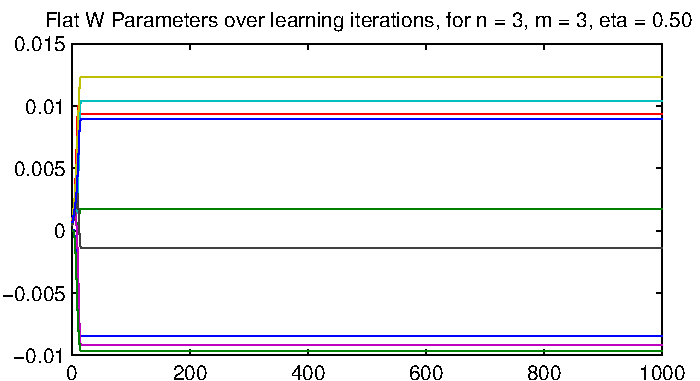
\includegraphics[width=0.48\textwidth]{../plots/learning-eta-5a.pdf}}
  \subfloat[$\eta$: .1]{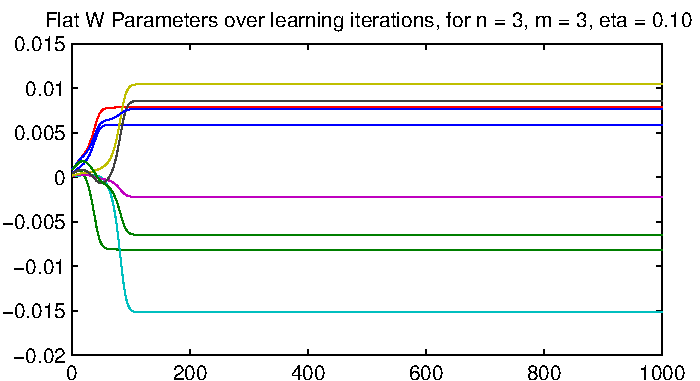
\includegraphics[width=0.48\textwidth]{../plots/learning-eta-1a.pdf}}
  \caption{$W$ convergence for large $\eta$.}
  \label{fig:eta5}
\end{figure}

\begin{figure}[H]
  \centering
  \subfloat[$\eta$: Run 1]{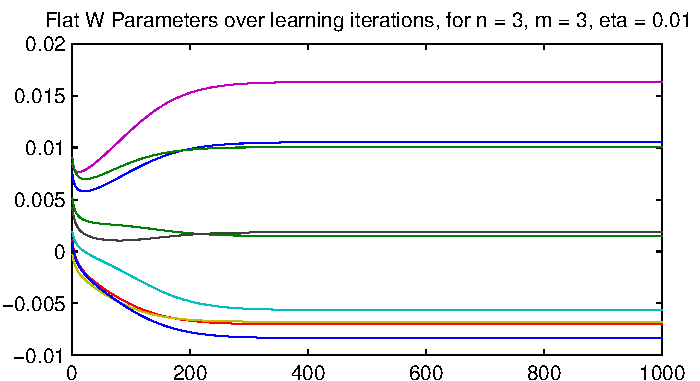
\includegraphics[width=0.48\textwidth]{../plots/learning-eta-01a.pdf}}
  \subfloat[$\eta$: Run 2]{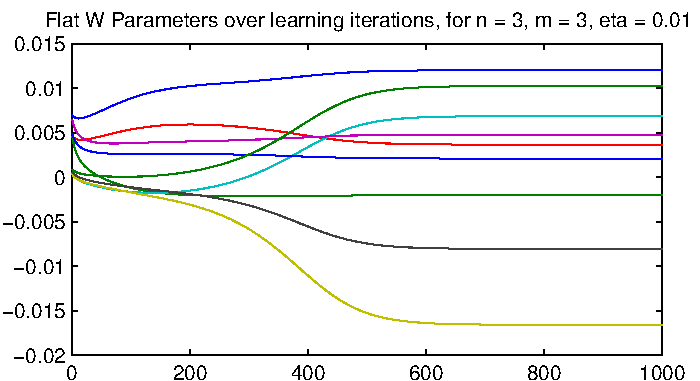
\includegraphics[width=0.48\textwidth]{../plots/learning-eta-01b.pdf}}
  \caption{$W$ convergence for $\eta$: 0.01.}
  \label{fig:eta01}
\end{figure}

\begin{figure}[H]
  \centering
  \subfloat[$\eta$: Run 1]{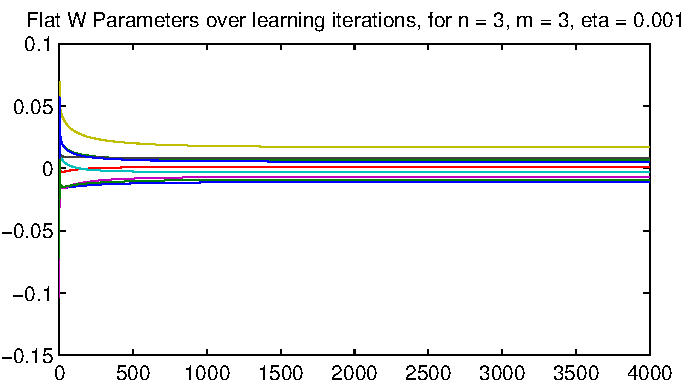
\includegraphics[width=0.48\textwidth]{../plots/learning-eta-001.pdf}}
  \caption{$W$ convergence for very small $\eta$ (but somewhat larger initial $W$).}
  \label{fig:eta001}
\end{figure}


\section{Evaluation}

Quantitative evaluation is somewhat arbitrary, since we have no recognized standard for calculating similarity between audio signals. For the purposes of evaluating between different runs in this particular homework, though, the best method I have come up with is to compare means of pairwise cosine similarity measures. That is, I compare a pair of audio signals (simple vectors) with each other using MATLAB's \texttt{pdist2} function with the `cosine' option. Each of these pairs produces one cosine similarity value, and I take the mean of these values to compare total similarity between, for example, all three input streams and all three inferred signals.

We can draw out simplified (smoothed) waveforms for each channel, mixture, and inferred output, as in Figure \ref{fig:a}.

% HW4 says, "See how well you can recover the original signals over several trials." You should evaluate the recovered signals visually, by plotting them, but also quantitatively. You can compute the quality of a reconstructed signal as the minimum distance to one of the original signals. (You have to do this because you don't know which reconstruction corresponds to which original.) 

\begin{figure}[H]
  \centering
  \subfloat[Original]{
    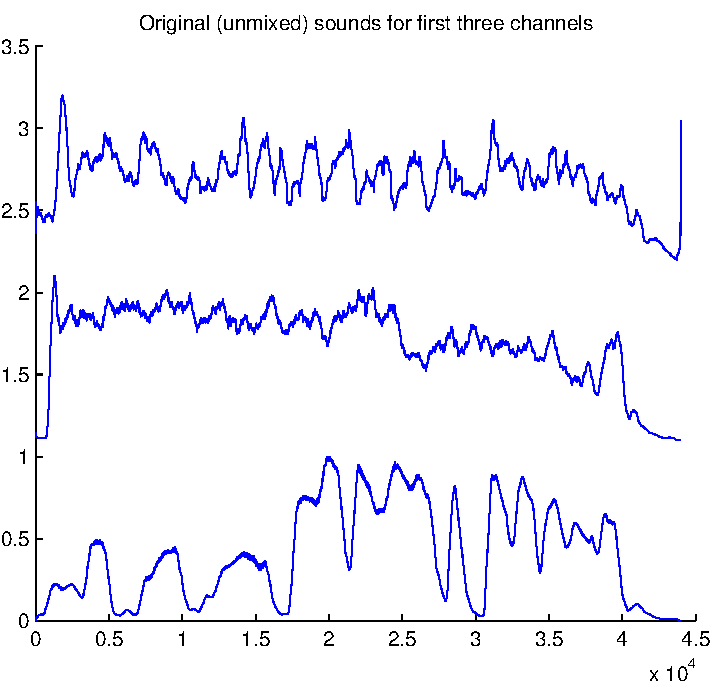
\includegraphics[width=0.31\textwidth]{../plots/U3.pdf}
  }\hfil
  \subfloat[Mixture]{
    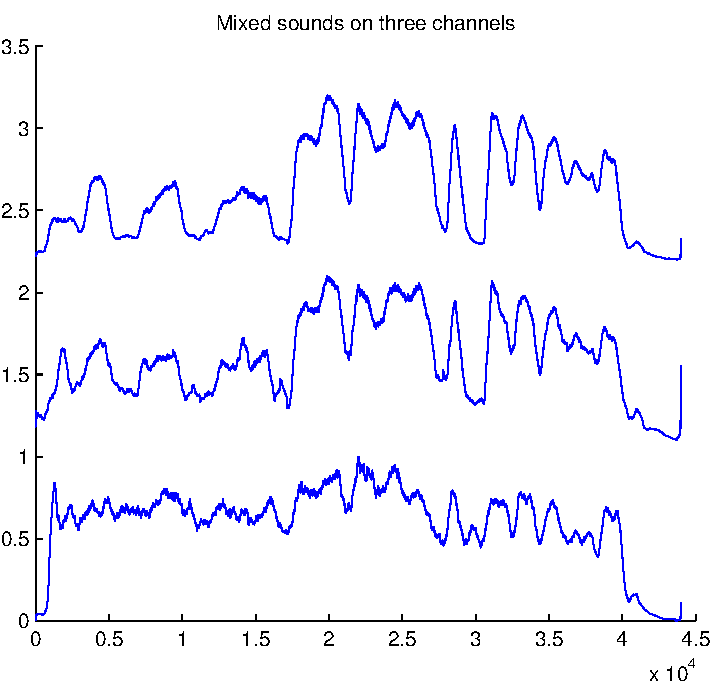
\includegraphics[width=0.31\textwidth]{../plots/X3.pdf}
  }\hfil
  \subfloat[Inference]{
    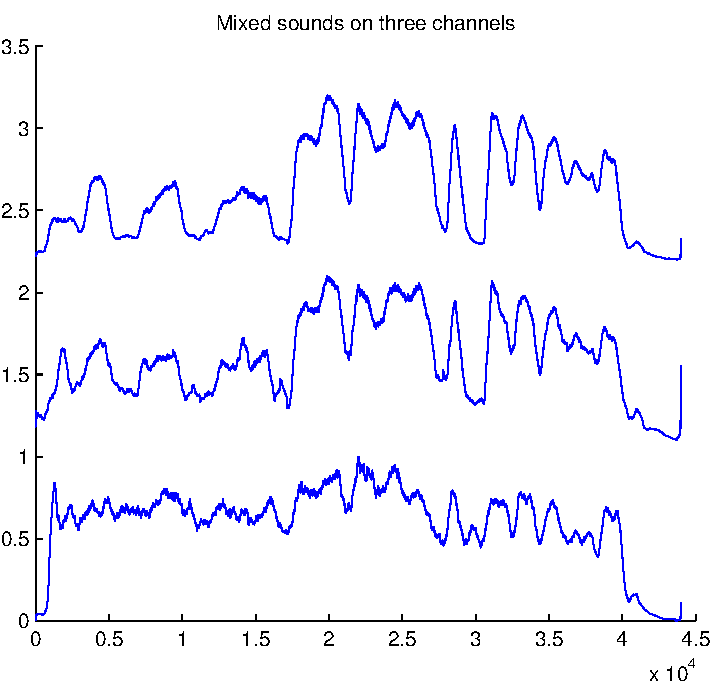
\includegraphics[width=0.31\textwidth]{../plots/X3.pdf}
  }
  \caption{Three channel input--three channel mixture.}
  \label{fig:a}
\end{figure}
However, it's hard to see exactly how these line up, so we can overlay the inferred channels over the original streams, as in Figure \ref{fig:b}. However, because this is an unsupervised task, we may very well get our groups in the wrong order, as in the graph on the left. So, we calculate the permutation with the closest similarity to the original data (on the right).

\begin{figure}[H]
  \centering
  \subfloat[Default]{
    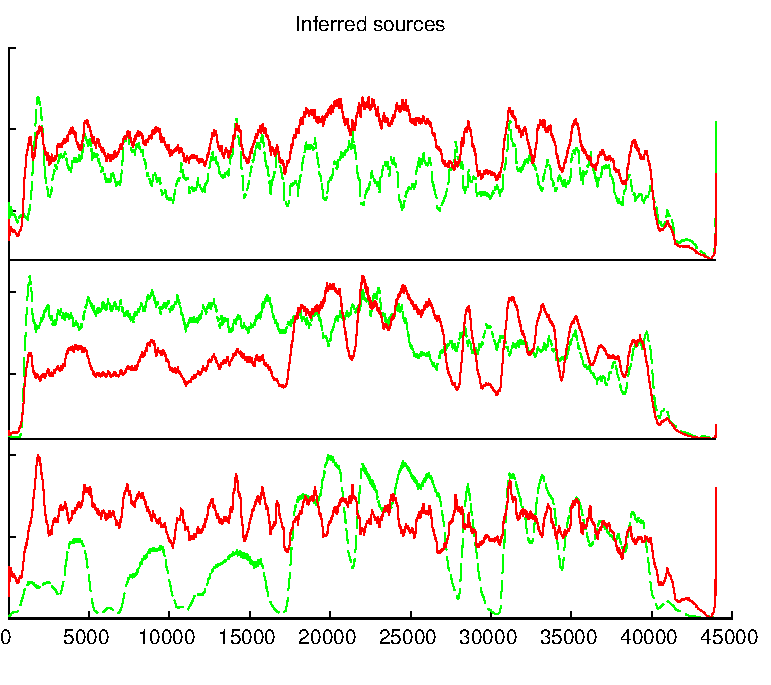
\includegraphics[width=0.47\textwidth]{../plots/mismatch3.pdf}
  }\hfil
  \subfloat[Corrected]{
    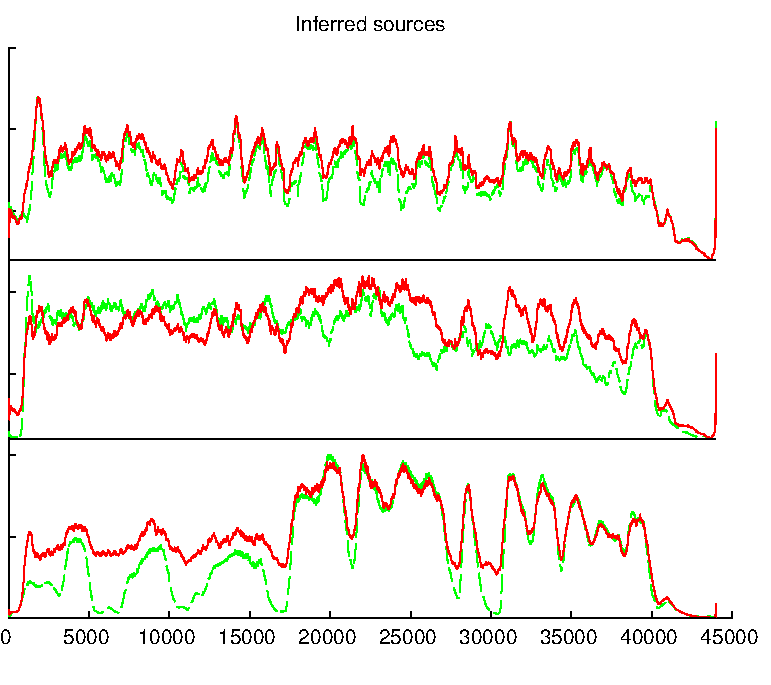
\includegraphics[width=0.47\textwidth]{../plots/goodmatch3.pdf}
  }
  \caption{Three channel input--five channel mixture. Green is original audio, red is inferred. The streams have been normalized, so the units of the vertical axis are irrelevant.}
  \label{fig:b}
\end{figure}
The (best case) total cosine similarity mean (after correction) for the three channels in Figure \ref{fig:b} is 0.218.

Using all five sources of audio signals, and mixing over five channels produced the plot in Figure \ref{fig:c}, for which the mean cosine similarity was 0.173.
\begin{figure}[H]
  \centering
  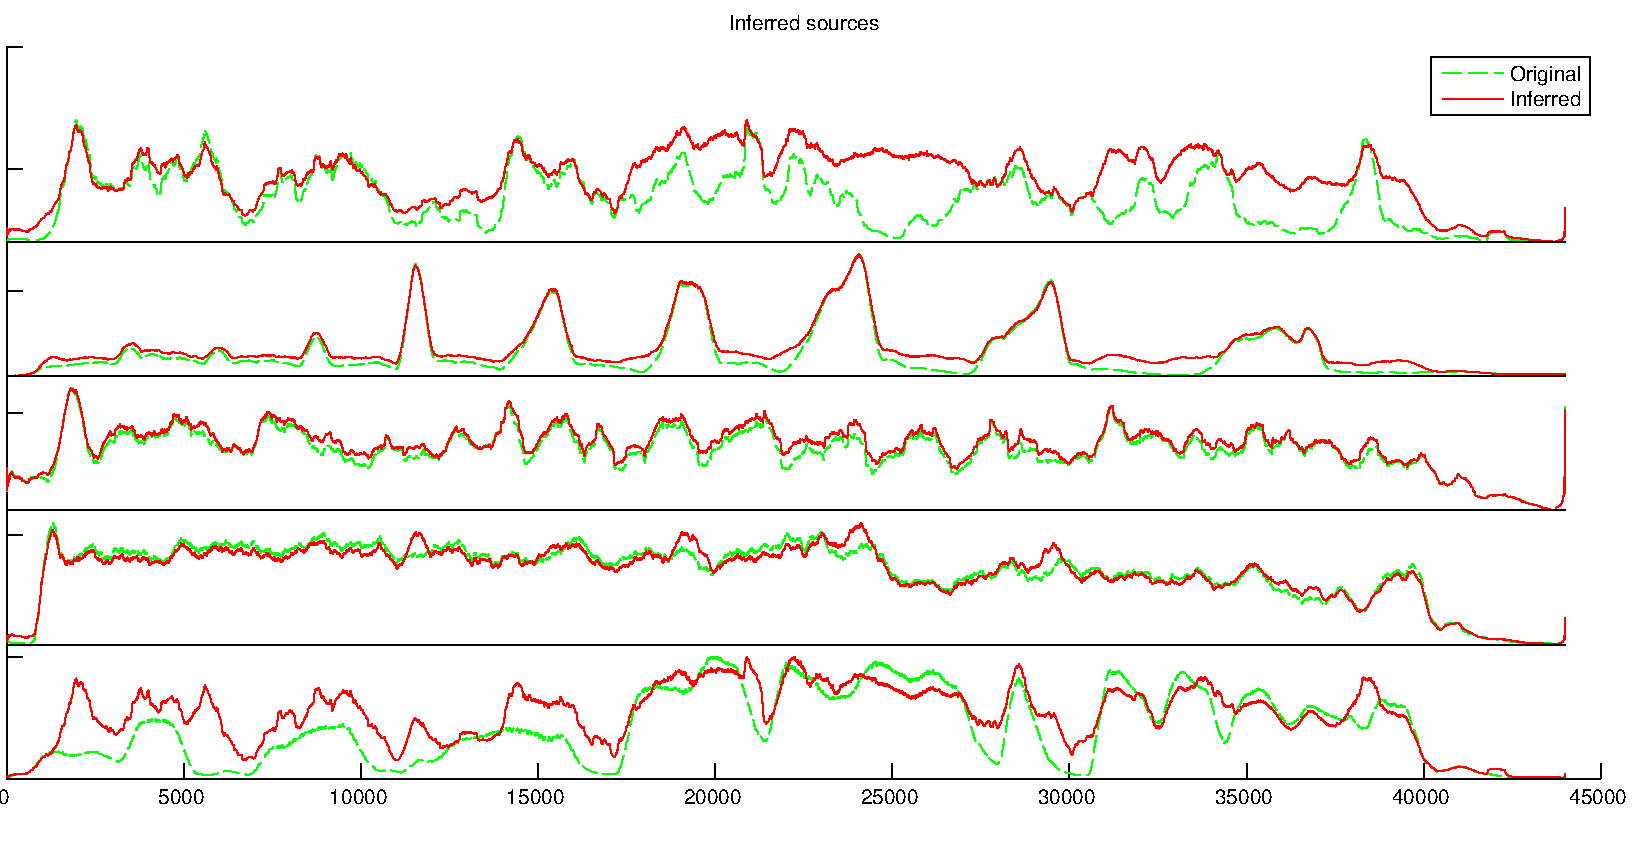
\includegraphics[width=\textwidth]{../plots/goodmatch5.pdf}
  \caption{Five channel input--five channel mixture.}
  \label{fig:c}
\end{figure}
In Figure \ref{fig:d}, I have printed out the inferences for 10 different runs over the same mixture, showing the amount of variance that can occur, i.e. the great many local minima that we can fall into.
\begin{figure}[H]
  \centering
  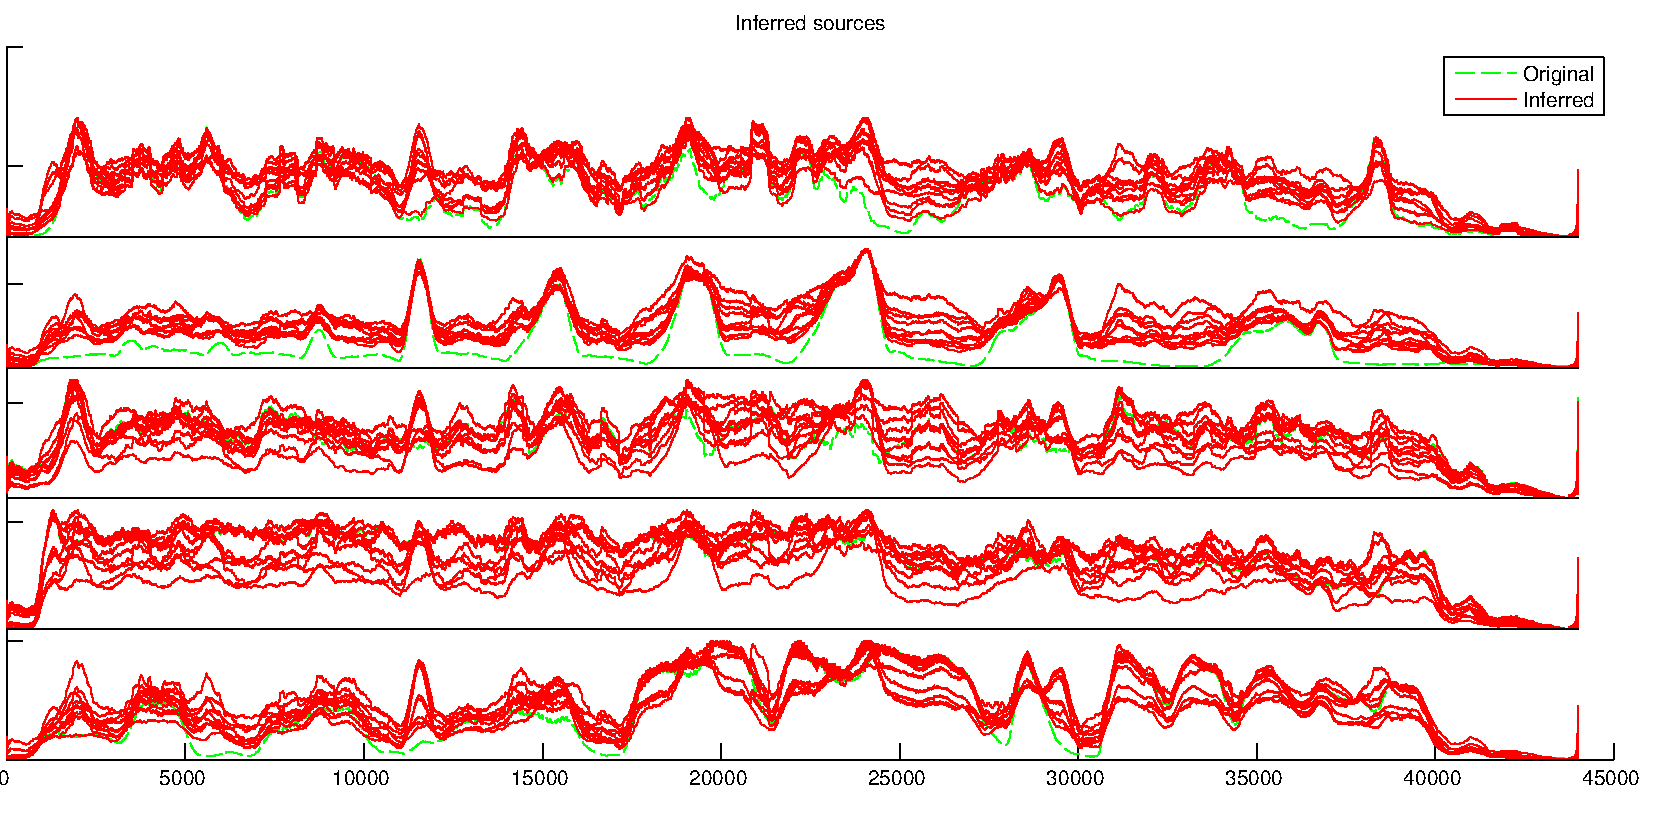
\includegraphics[width=\textwidth]{../plots/5channels10.pdf}
  \caption{Five channel input--five channel mixture, 10 runs.}
  \label{fig:d}
\end{figure}
I've been pretty generous so far, my mixture matrix has not been entirely random -- I've skewed it so that each mixture channel will receive signal from primarily one input (about a 1:1 ratio---half one channel, half the others). But a fully randomized mixture matrix doesn't actually change things very much; the algorithm is still very good at inferring the sources:
\begin{figure}[H]
  \centering
  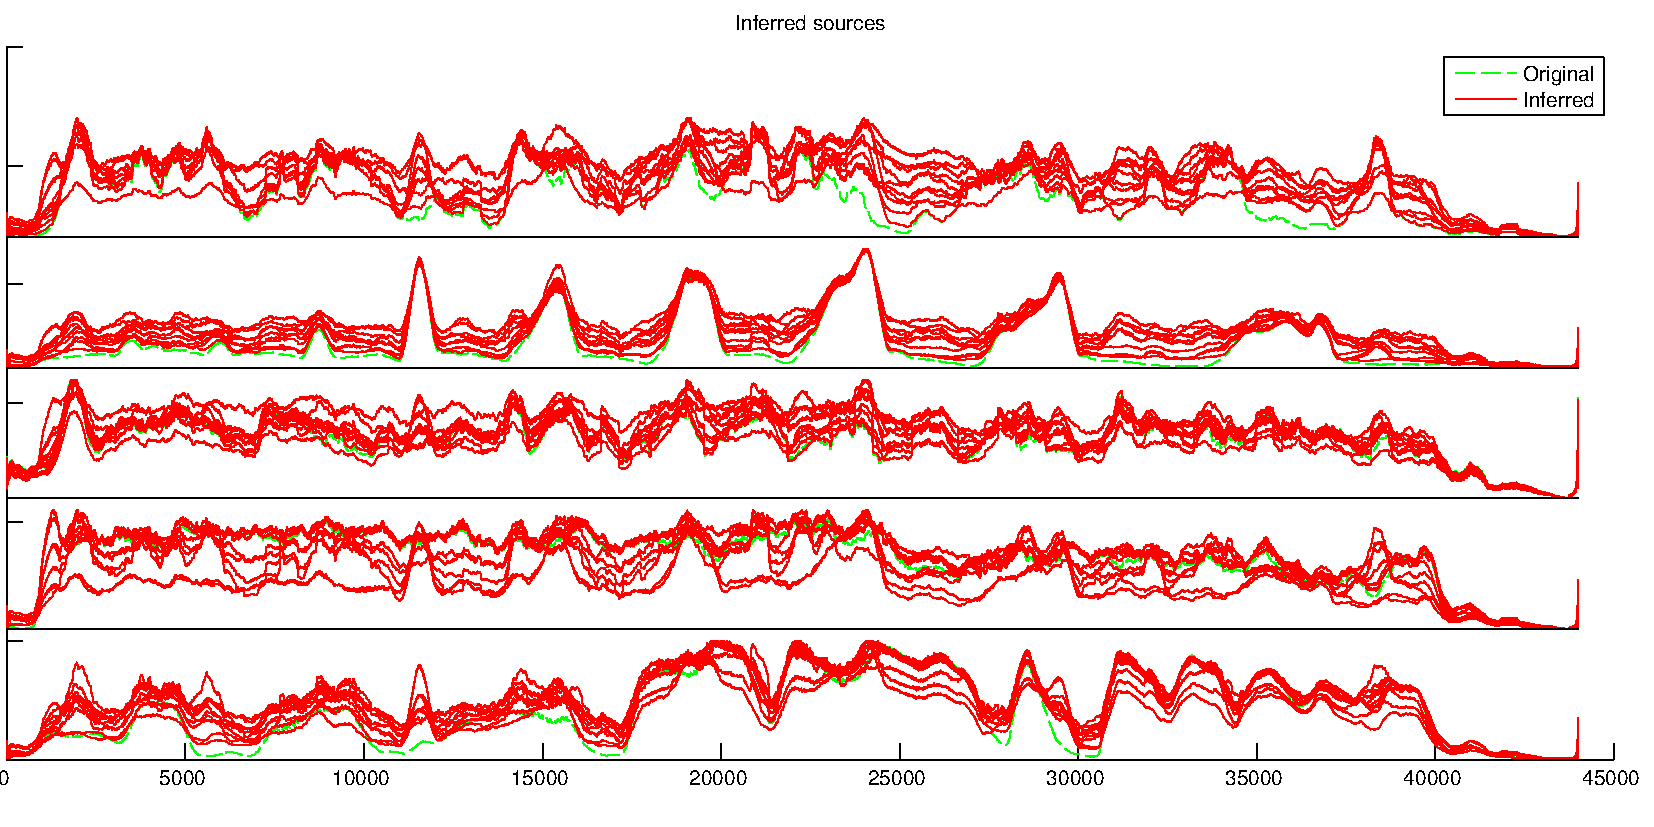
\includegraphics[width=\textwidth]{../plots/5channels10b.pdf}
  \caption{Five channel input--five channel mixture, 10 runs, fully randomized.}
  \label{fig:e}
\end{figure}
Most of the work above has mixed the original channels over an equivalent number of mixed channels ($A$ has been square). The variance is certainly more compact with a greater number of channels, as we might expect, but not extraordinarily so (see Figure \ref{fig:f}).
\begin{figure}[H]
  \centering
  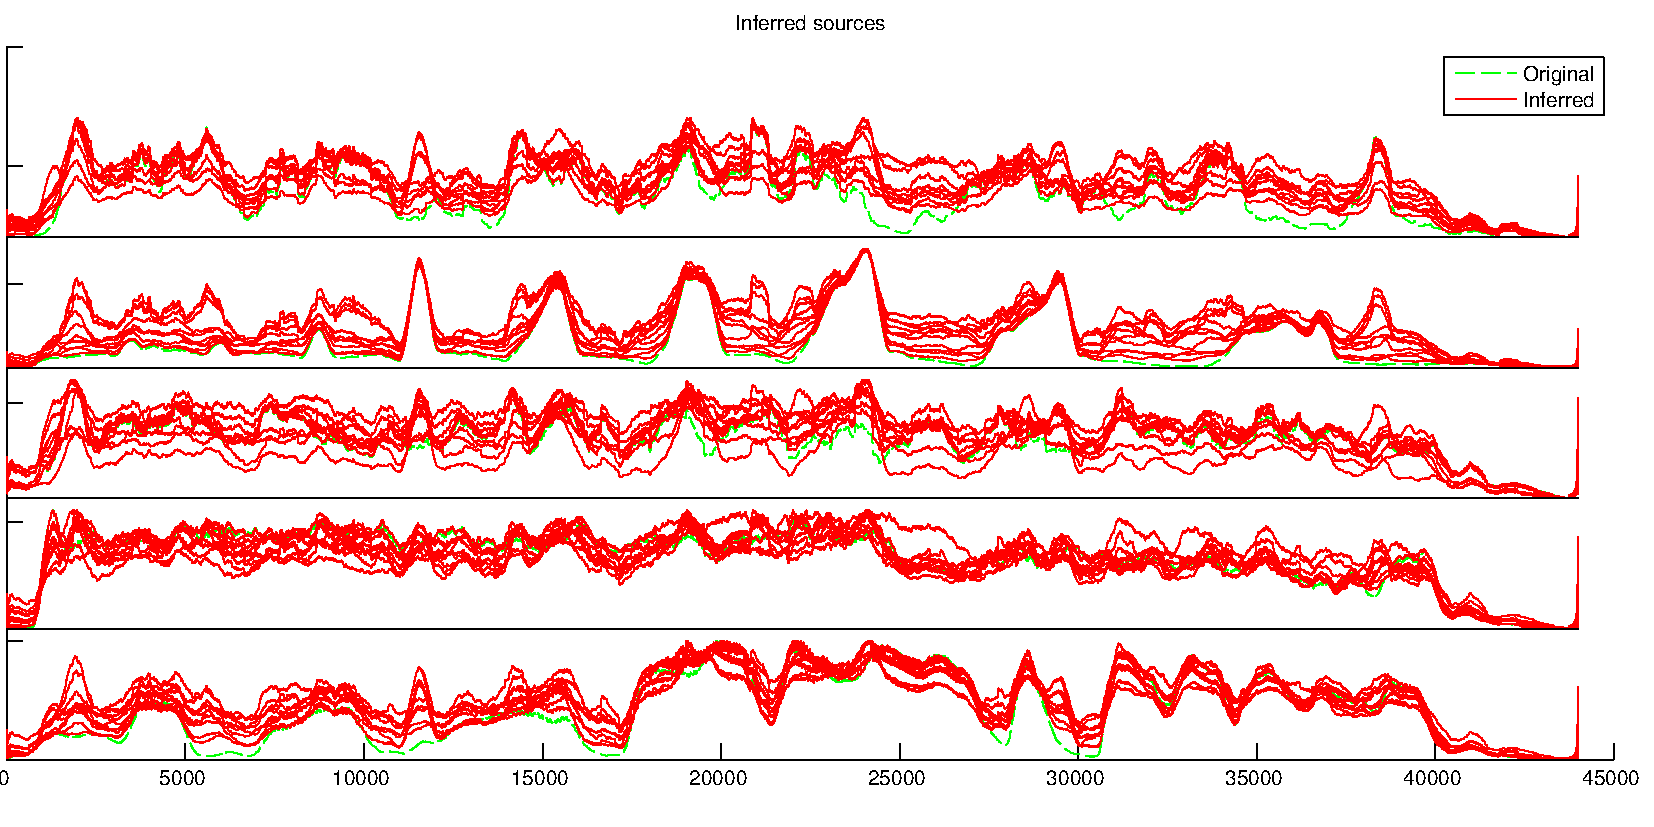
\includegraphics[width=\textwidth]{../plots/5channels10-25mix.pdf}
  \caption{Five channel input--25 channel mixture, 10 runs, fully randomized.}
  \label{fig:f}
\end{figure}
Finally, the result of mixing five input channels into just two `microphones' has pretty drastic results, as we might have predicted. The results, as you can see in Figure \ref{fig:g}, are considerably off. And while we can tell the algorithm that there are five original source signals, it cannot produce more than two basic shapes (rows 1, 2, and 5, and then 3 and 4, counting from the top).
\begin{figure}[H]
  \centering
  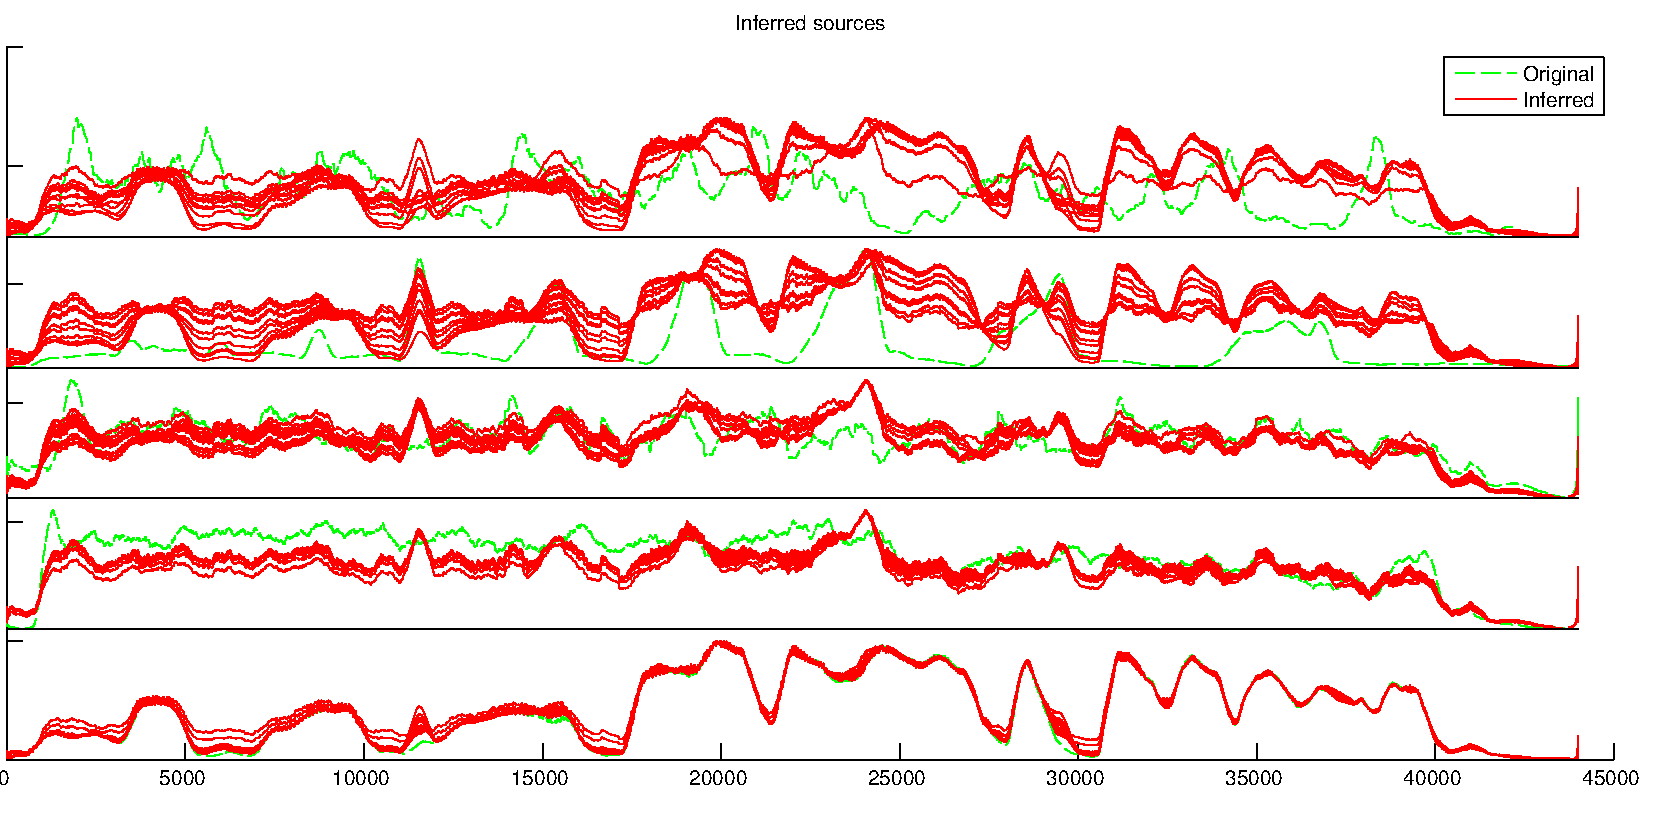
\includegraphics[width=\textwidth]{../plots/5channels10-2mix.pdf}
  \caption{Five channel input--two channel mixture, 10 runs, fully randomized.}
  \label{fig:f}
\end{figure}

\section{Notes}

One problem I came up against was that if my initial random values of $W$ were not small enough, my $\Delta W$ would grow too large and my $W$ values would quickly spiral out of control, growing too large for MATLAB to handle within six or seven iterations.

The algorithm is best (least random) at discerning the source for areas of particular volume. The fourth row in the original data (the wheezing laugh), is the most retrievable of any of the signals.



% \begin{figure}[H]
%   \centering
%   \subfloat[asdasdasdas]{
%     \makebox[0.3\textwidth]{
%       \includegraphics[height=0.3\textwidth]{.pdf}
%     }
%   }
%   \subfloat[Using 100 training images]{
%     \makebox[0.3\textwidth]{
%       \includegraphics[height=0.3\textwidth]{.pdf}
%     }
%   }
%   \caption{The first }
%   \label{fig:a}
% \end{figure}



\end{document}

